\section{MIPS instruction execution}

Each instruction within the MIPS subset can be executed within a maximum of five clock cycles, as outlined below:
\begin{enumerate}
    \item \textit{Instruction fetch cycle}: 
        \begin{itemize}
            \item Transfer the content of the program counter register to the instruction memory and retrieve the current instruction.
            \item Update the program counter to the next sequential address by incrementing it by 4 (since each instruction occupies 4 bytes).
        \end{itemize}
    \item \textit{Instruction decode and register read cycle}: 
        \begin{itemize}
            \item Decode the current instruction using fixed-field decoding.
            \item Access the register file to read one or two registers as specified by the instruction fields.
            \item Perform sign-extension of the offset field of the instruction if necessary.
        \end{itemize}
    \item \textit{Execution cycle}: 
        \begin{itemize}
            \item For register-register ALU instructions, the ALU performs the specified operation on the operands retrieved from the register file (RF).
            \item For register-immediate ALU instructions, the ALU performs the specified operation on the first operand retrieved from the RF and the sign-extended immediate operand.
            \item For memory reference instructions, the ALU computes the effective address by adding the base register and the offset.
            \item For conditional branches, it compares the two registers read from the RF and calculates the potential branch target address by adding the sign-extended offset to the incremented program counter (PC).
        \end{itemize}
    \item \textit{Memory access}:
        \begin{itemize}
            \item Load instructions entail a read access to the data memory using the effective address.
            \item Store instructions require a write access to the data memory using the effective address to store the data from the source register read from the RF.
            \item Conditional branches may update the content of the PC with the branch target address if the conditional test evaluates to true.
        \end{itemize}
    \item \textit{Write-back cycle}: 
        \begin{itemize}
            \item Load instructions write the data retrieved from memory into the destination register of the RF.
            \item ALU instructions store the ALU results into the destination register of the RF.
        \end{itemize}
\end{enumerate}
\begin{figure}[H]
    \centering
    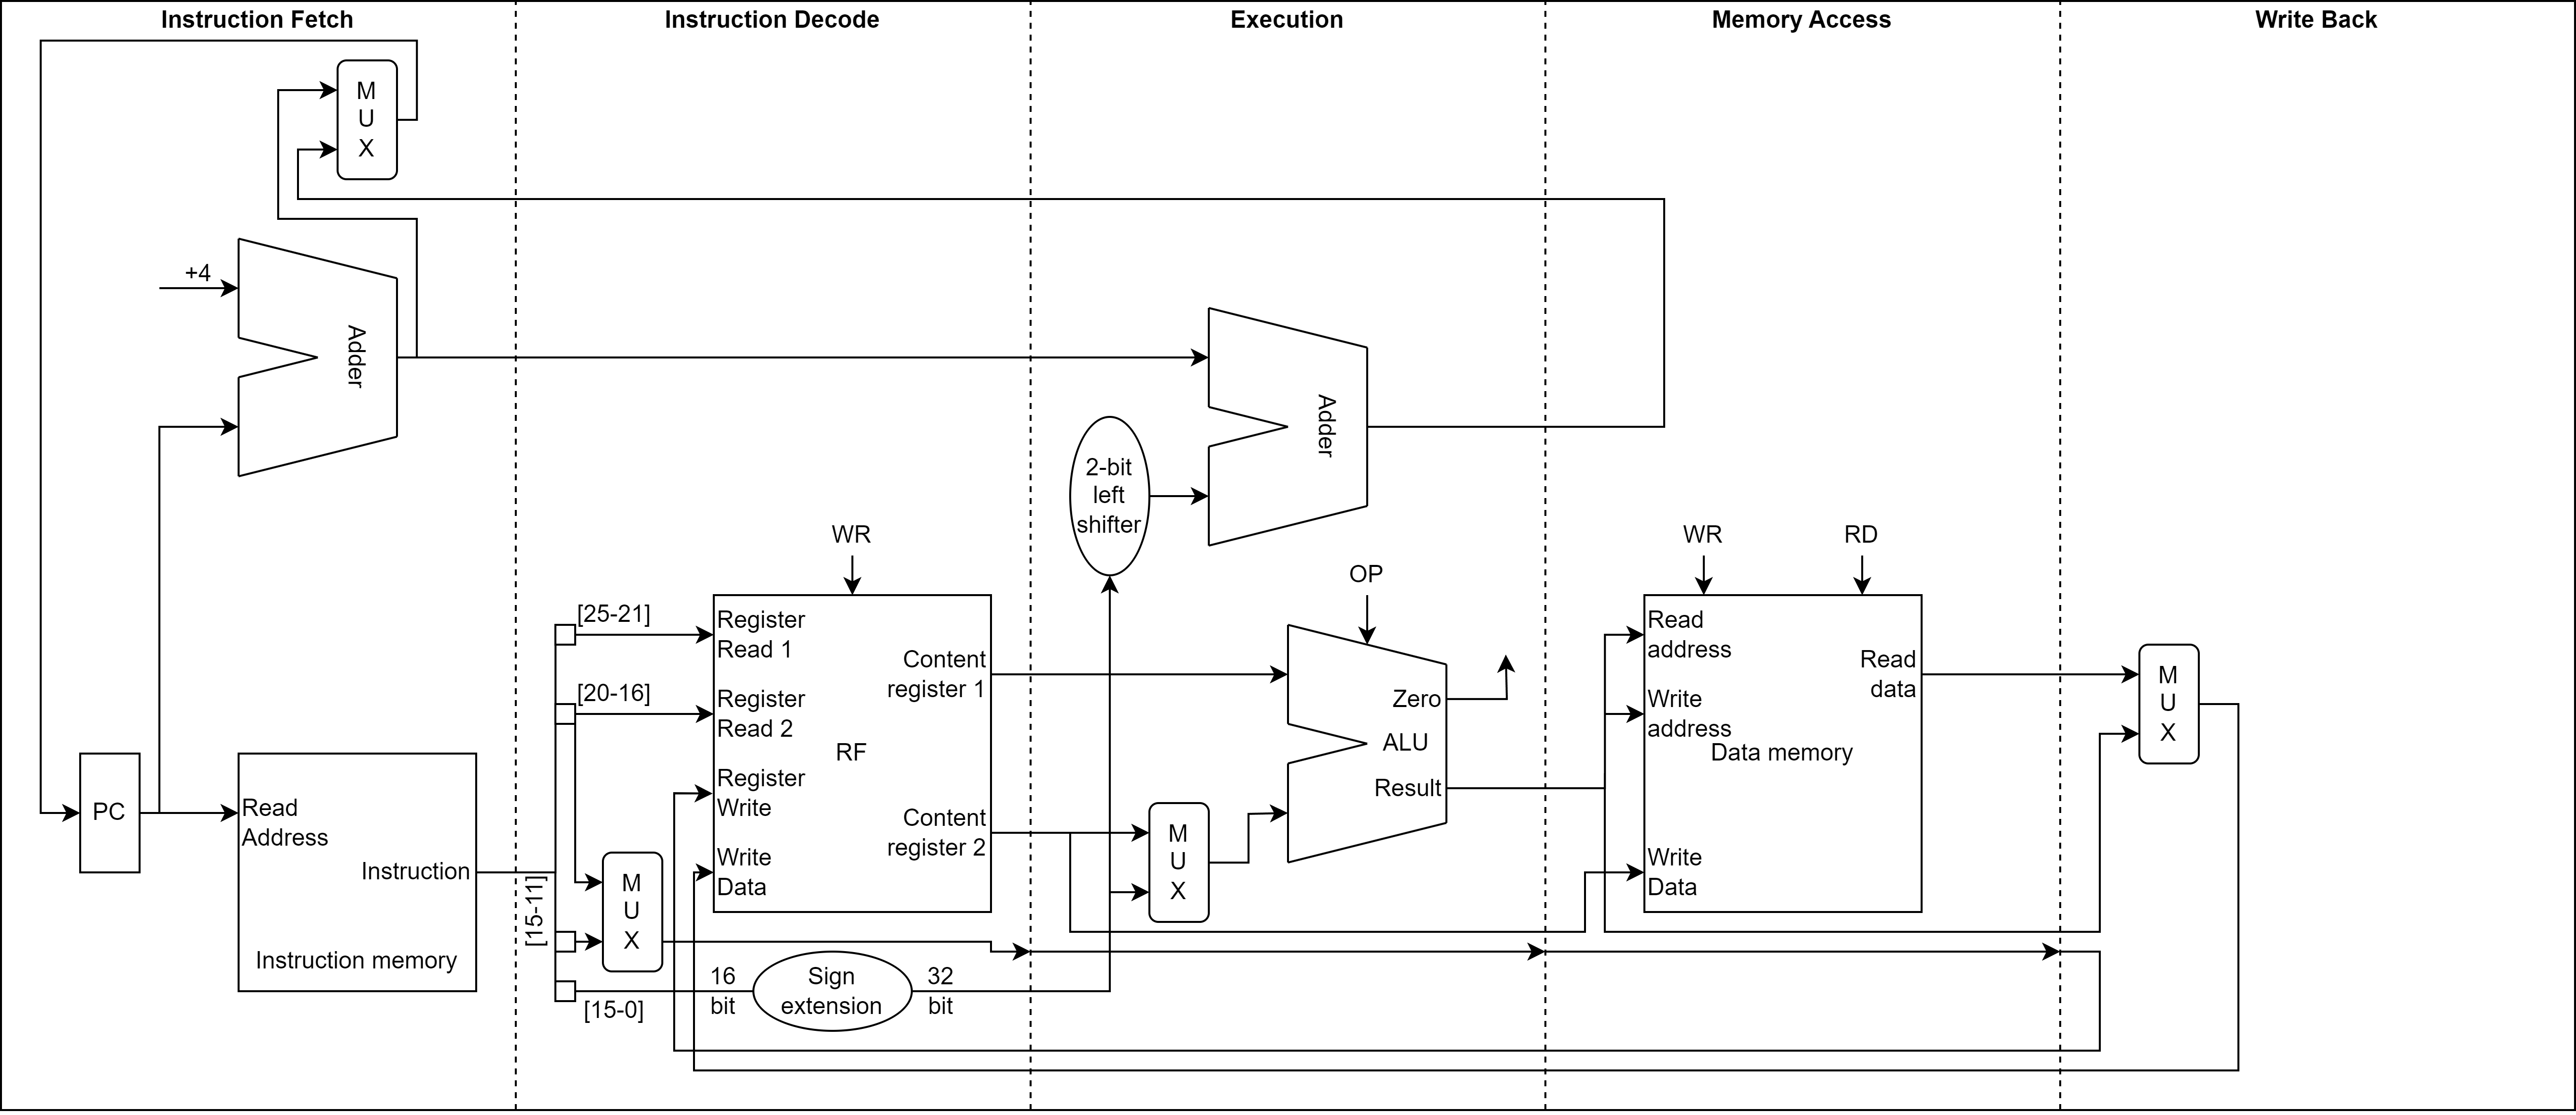
\includegraphics[width=1\linewidth]{images/mips.png}
    \caption{MIPS CPU architecture}
\end{figure}
Below are the durations of each instruction:
\begin{table}[H]
    \centering
    \begin{tabular}{l|ccccc|c}
    \makecell[l]{\textbf{Instruction} \\ \textbf{type}} & \makecell{\textbf{Instruction} \\ \textbf{memory}} & \makecell{\textbf{Register} \\ \textbf{read}} & \makecell{\textbf{ALU} \\ \textbf{operations}} & \makecell{\textbf{Data} \\ \textbf{memory}} & \makecell{\textbf{Write} \\ \textbf{back}} & \makecell{\textbf{Total} \\ \textbf{latency}} \\ \hline
    ALU instruction           & 2                           & 1                      & 2                       & 0                    & 1                   & $6ns$                  \\
    Load                      & 2                           & 1                      & 2                       & 2                    & 1                   & $8ns$                  \\
    Store                     & 2                           & 1                      & 2                       & 2                    & 0                   & $7ns$                  \\
    Conditional branch        & 2                           & 1                      & 2                       & 0                    & 0                   & $5ns$                  \\
    Jump                      & 2                           & 0                      & 0                       & 0                    & 0                   & $2ns$                 
    \end{tabular}
\end{table}

The duration of each clock cycle is determined by the critical path established by the load instruction, denoted as $T = 8 ns$ (equivalent to a frequency of $f = 125 MHz$).
We assume a single-clock cycle execution for each instruction, wherein each module is utilized once within a cycle. 
Modules utilized more than once within a cycle necessitate duplication for efficiency. 
Furthermore, to ensure separate functionality, an instruction memory distinct from the data memory is required.

Certain modules must be duplicated, while others are shared across different instruction flows.
To facilitate sharing a module between two distinct instructions, a multiplexer is utilized.
This device enables multiple inputs to access a module and allows the selection of one input among several based on the configuration of control lines.

In the multi-cycle implementation of CPU, the execution of instructions spans across multiple cycles, with MIPS typically utilizing five cycles. 
The fundamental cycle is shorter at $2 ns$, leading to an instruction latency of $10 ns$.
Key aspects of the multi-cycle CPU implementation include:
\begin{itemize}
    \item Each phase of instruction execution necessitates a clock cycle.
    \item Modules can be utilized multiple times per instruction across different clock cycles, allowing for potential module sharing.
    \item Internal registers are required to retain values for subsequent clock cycles. These registers store data to be utilized in future stages of the instruction execution process.
\end{itemize}